\section{Results}
\subsection{Poiseuille Flow}
\subsubsection{Test of the Basic Algorithm}

The results of the grid convergence study are shown in Fig. \ref{fig:ema1}.
The double logarithmic axis shows the dependency of the computed relative $l_2$-error norm
with respect to the grid resolution.

On this scale, the FD4 has a linear decreasing error.
For the smallest resolution $N=8$ the error is of order $10^{-3}$,
in contrast to the highest resolution $N=256$ with an error of order $10^{-6}$.
A convergence rate of the error  was computed  according to $\lambda\approx -2.26$.
Hence, it can be said that the accuracy of the method is above secnd order for this test case,
which is in contradiction with the theory assuming a 4th order.
The error of the second order finite difference scheme is of the order $10^{-8}$.
The value is approximately constant and does not depend on the grid resolution.

\begin{figure}[!bp]
    \centering
    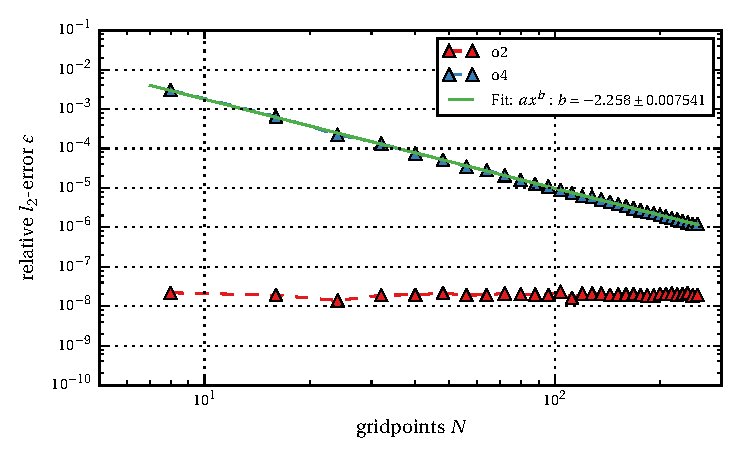
\includegraphics{gfx/immersed_boundary/poiseuille_flow/1_default/relative_l2error.pdf}
    \caption{Relative $l_2$-error for FD2 and FD4 methods with the basic algorithm without the use of an immersed boundary.\label{fig:ema1}}
\end{figure}


\subsubsection{Test of the Volume Penalization Method}

The first simulation was  a parameter study with variable Reynolds number and damping coefficient.
A first impression of the influence of the damping coefficient $J$ is given by the velocity profiles of the numerical solution.
For varying $J$ and $Re=500$, this is exemplarily shown in Fig. \ref{fig:vp_flow}.
 It can be noted that with an decrease of $J$, the numerical solution converges against the theoretical one.
Furthermore, it can be seen that the quadratic part of the velocity profile,
inside of the fluid domain ($0.5\leq z \leq 1.5$), is independent of the damping constant $J$.
Merely a slight offset at the boundaries creates a constant shift upwards of the velocity profile.
In the masked area of the volume a decrease in velocity is visible which could  eventually be described by an
exponential law.

\begin{figure}[!t]
  \centering
  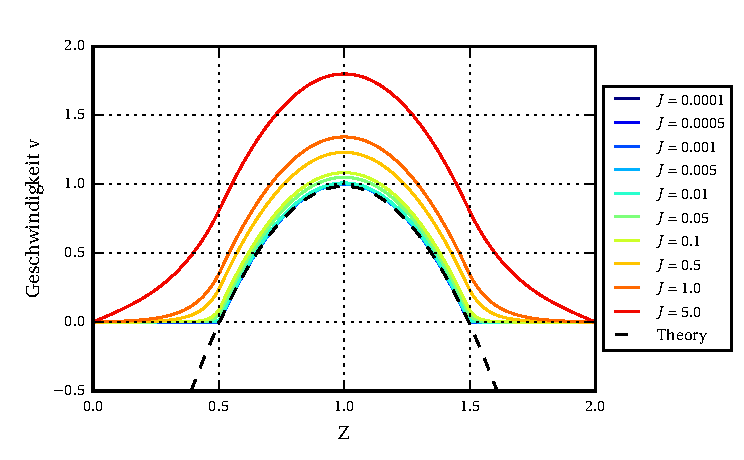
\includegraphics{gfx/immersed_boundary/poiseuille_flow/2_vp/vp_profile.pdf}  \caption{\label{fig:vp_flow}
    Velocity profile of the numerical solution with variable $J$ and $\Rey = 500$.}
\end{figure}

For an error estimation the relative $l_2$-error was computed, the results are shown in Fig. \ref{fig:vp_error}.
On the left side of the plot the relative error is plotted against the damping coefficient and the Reynolds number is
varied over a color scale. On the right side both variables ($J$ and $\Rey$) are switched.

\begin{figure}[!b]
  \centering
  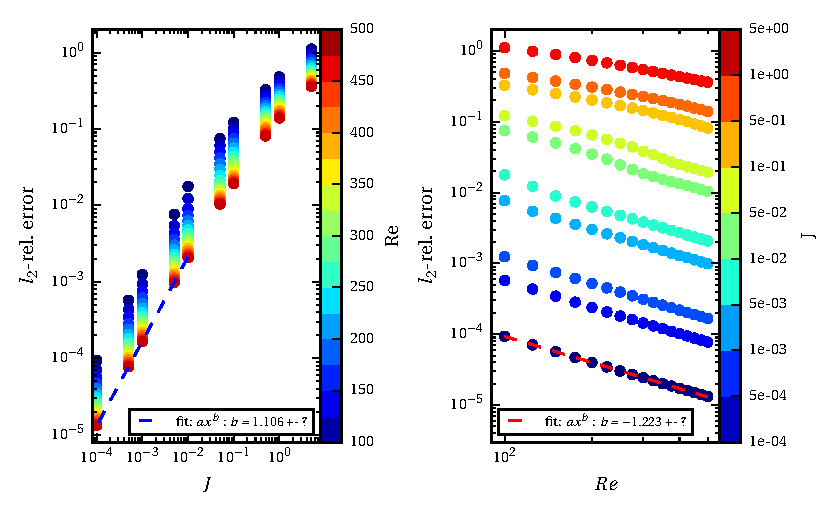
\includegraphics{gfx/immersed_boundary/poiseuille_flow/2_vp/vp_error.pdf}  \caption{\label{fig:vp_error}
    Relative $l_2$-error for variable damping rate $\nu$ and Reynolds number $Re$.}
  \centering
  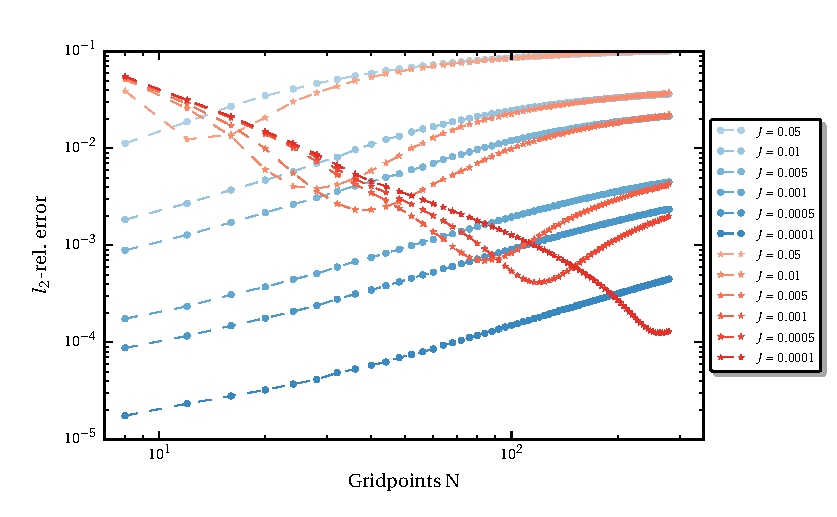
\includegraphics{gfx/immersed_boundary/poiseuille_flow/2_vp/vp_convergence.pdf}
  \caption{Relative $l_2$ error for variable damping rate $J$, for VP-FD2 (blue) and VP-FD4 (red) methods.}
    \label{fig:pflowvali_vp_conv}
\end{figure}


A decrease in the damping coefficient $J$ results in a decrease of the error of about four orders, from $10^{-1}$ to $10^{-5}$.
With a change of the Reynolds number from $500$ to $100$ the error decreases about one order.
It can be noticed that with a decrease of $\Rey$ or $J$ the error decreases linearly in the log-log space.
For a small damping ($J>10^{-3}$) a breakdown of the linear relation can be observed.
This is an error resulting from the numerical setup.
The damping in the masking area is so weak that the flow reaches the  boundaries of the numerical domain.
This is not the case for $J<10^{-3}$ since the velocity profile is zero before it reaches the boundaries.
A linear fit in the log-log space gives a  decay rate of about $1.106$ for  $J$ and about $-1.223$ for $\Rey$.

The second part of the test was a grid convergence study with a constant Reynolds number, variable $J$ and grid resolution $N$.
The results are shown in Fig. \ref{fig:pflowvali_vp_conv}.
It can be noticed that a decrease in $J$ creates a shift in the error profile to overall smaller values.
However, it is also noticable that the error of the FD2 method increases together with the resolution.

The error convergence for the FD4 method is even less understandable.
With increasing resolution  a decrease into a minimum which is followed by an increase can be observed.
The position of the minimum is shifted to the right with an decrease of $J$.
For a constant $J>10^{-4}$ it is visible that the error for both methods converges against a
the same error  with an increase in the resolution.

\clearpage

\subsubsection{Test of the Direct Forcing Method}

The results of this grid convergence study for the DF method
are similar to the results of the basic implementation, except the DF-FD4 method has a larger error.
A plot of the relative $l_2$-error can be found in the Appendix in Fig.\ref{fig:vali_pflow_3gc}.
The FD4 method has a linear decreasing error in the log-log space.
For the smallest resolution $N=8$ the error is of order $10^{-2}$,
in contrast to the highest resolution $N=256$, with an error of order $10^{-4}$.
The convergence rate is about $\lambda\approx1.267$.
Hence, it can be said that the accuracy of the method is above first order for this test case.
The error of the second order finite difference scheme is of the order $10^{-8}$.
The value is approximately constant and not depend of the grid resolution.

\subsection{Hagen-Poiseuille Flow}

\subsubsection{Grid Convergence Study}

The results of the grid convergence study are shown from Fig. \ref{vali:hp_flow_gc_vp} to Fig. \ref{vali:hp_flow_gc_all}.
For a better overview the results are distributed into four plots.
For all methods (except IP+DF FD4) an approximately linear decrease in the double logarithmic space can be observed.

In Fig. \ref{vali:hp_flow_gc_vp} the relative $l_2$-error is shown for different VP methods.
For the default VP-method with FD2 and FD4 the error convergence rate is about $\lambda=1.17$.
The FD4 has a slightly smaller error than the FD2 method.
The optional use of the VF-method improves the error convergence is about $\lambda=1.65$,
here the FD2 method has a slightly smaller error.
It can be noted that the overall error is smaller ($\approx 10^{-2}$ for $N=100$)
when using the VP-VF-method in comparison to the VP-method ($\approx2\cdot 10^{-2}$ for $N=100$)

In Fig. \ref{vali:hp_flow_gc_df} the relative $l_2$-error is shown for different DF methods.
For the default DF-method with FD2 and FD4 the error convergence rate is about $\lambda=1.2$.
Again the FD4 method has a smaller error than the FD2 method.
The optional use of the VF-method improves the error convergence to about $\lambda=1.4$,
which is worse in comparison to the VP-method. The FD2 method has a smaller error than the FD4 method when using VF.
In comparison to the DF-method ($\approx2\cdot 10^{-2}$ for $N=100$),
the overall error is smaller ($\approx 1.5 \cdot 10^{-2}$ for $N=100$) for the DF-VF-method.

In Fig. \ref{vali:hp_flow_gc_ip} the relative $l_2$-error is shown for different IP methods.
For the IP FD4 method the decay rate is about $\lambda=1.4$.
For the IP FD2 and IP+DF FD2 method the errors are identical, the decay rate is about $\lambda=2.4$
The IP+DF FD4 method is numerically not stable and therefore not shown.
From the interpolation methods the IP FD2 method gives the smallest error  ($\approx 5 \cdot 10^{-5}$ for $N=100$).

Finally Fig. \ref{vali:hp_flow_gc_all} shows the methods  with the best convergence
rates from the different DF, VP and IP methods in one plot.
In summary, it can be said that the overall convergence rate of the IP FD2 method is of one order better
than the VP-VF and DF-VF methods. The relative error of the interpolation method ranges
between one and two order of magnitudes below all other methods.

\begin{figure}[!bp]
  \begin{minipage}[c]{0.45\textwidth}
      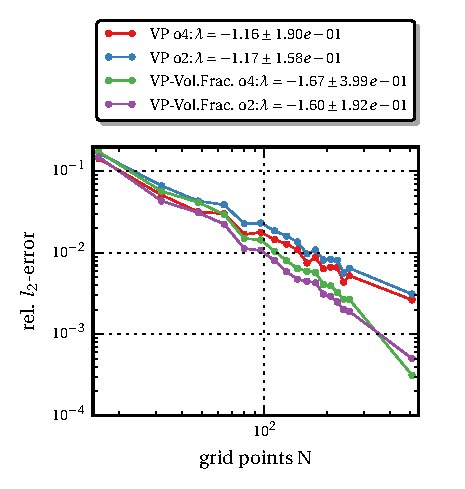
\includegraphics{gfx/immersed_boundary/hpflow/theo/vp.pdf}
      \caption{\label{vali:hp_flow_gc_vp}
          Relative $l_2$-error for different Volume-Penalization methods.}
  \end{minipage}
  \hfill
  \begin{minipage}[c]{0.45\textwidth}
      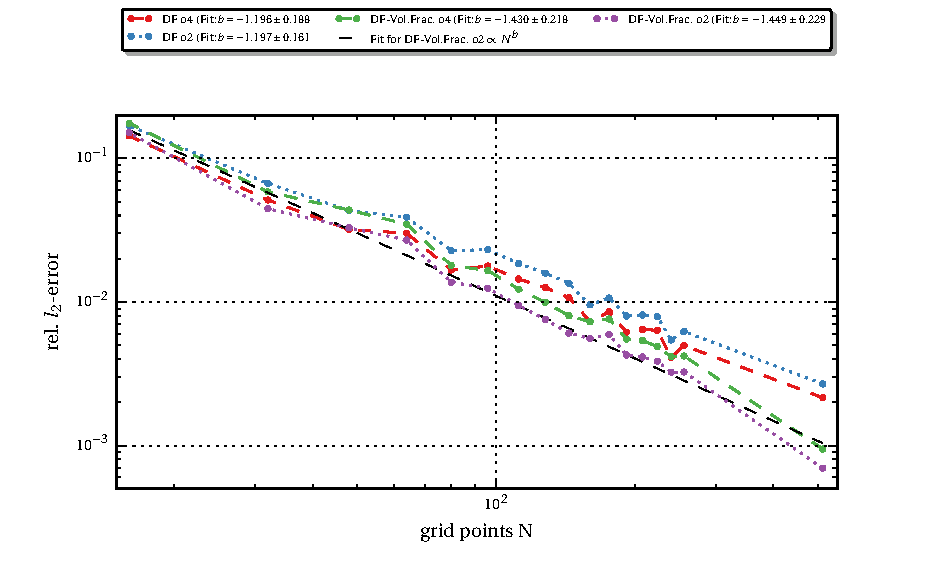
\includegraphics{gfx/immersed_boundary/hpflow/theo/df.pdf}
      \caption{\label{vali:hp_flow_gc_df}
          Relative $l_2$-error for different Direct-Forcing methods.}
  \end{minipage}
  \begin{minipage}[c]{0.45\textwidth}
      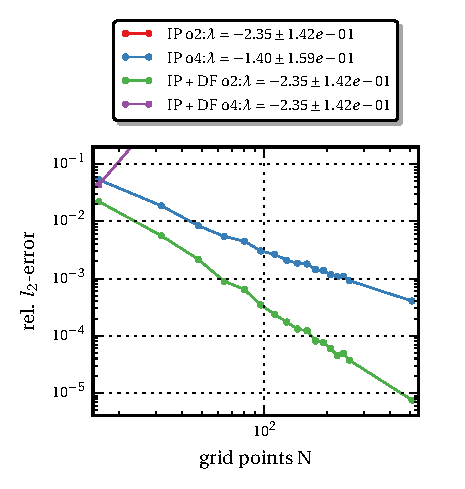
\includegraphics{gfx/immersed_boundary/hpflow/theo/ip.pdf}
      \caption{\label{vali:hp_flow_gc_ip}
          Relative $l_2$-error for different Interpolation methods.}
  \end{minipage}
  \hfill
  \begin{minipage}[c]{0.45\textwidth}
      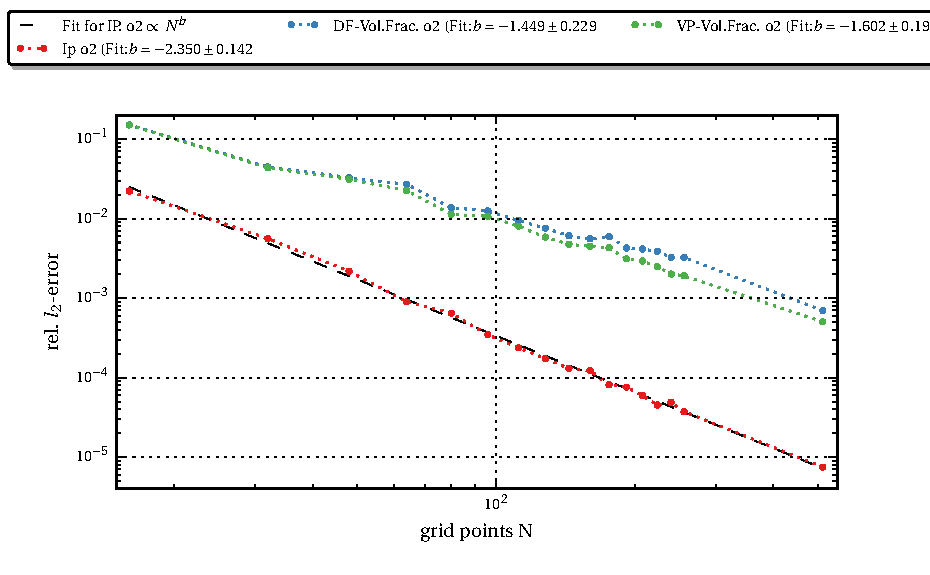
\includegraphics{gfx/immersed_boundary/hpflow/theo/all.pdf}
      \caption{\label{vali:hp_flow_gc_all}
          Relative $l_2$-error for the methods with the smallest error in comparison.}
  \end{minipage}
\end{figure}

\subsubsection{Long-Term Simulations}

The long-term simulations were performed in order to test the numerical stability and the conservation of mass.
For all methods these simulations were numerically stable, except the IP FD4 method.
The density was averaged over the fluid domain by

\begin{align}
    \label{vali:density_calc}
    \left<\rho(t)\right> = \frac{\int_V \dif V \rho(x,y,z)}{\int_V \dif V} =
    \frac{1}{N}\left(\sum_{i,j,k}^{N_x, N_y, N_z} \rho_{i,j,k}\right).
\end{align}


For all FD2 methods the averaged density is zero. This indicates that the total mass flux through the
fluid domain boundaries is zero.
It can be noticed that for all FD4 methods oscillations in the density emerge.
For the VP-VF-FD4 method this is exemplarily shown in Fig.  \ref{hpflow:results_long_ts}.
The profiles of the other FD4 methods are shown in Appendix \ref{fig:hpflow_allgc_theo}.

Finally in Fig. \ref{hpflow:results_long_example} the averaged density with respect to the simulation time is shown for the
FD4 methods.  For the VP and DF methods the density increases to above $5\cdot10^{-5}$.
The VF methods have a decrease in density, remaining within the order $10^{-4}$.
For all FD4 methods a change in the averaged density is followed by a saturation.

\begin{figure}[!bp]
  \begin{minipage}[c]{0.45\textwidth}
      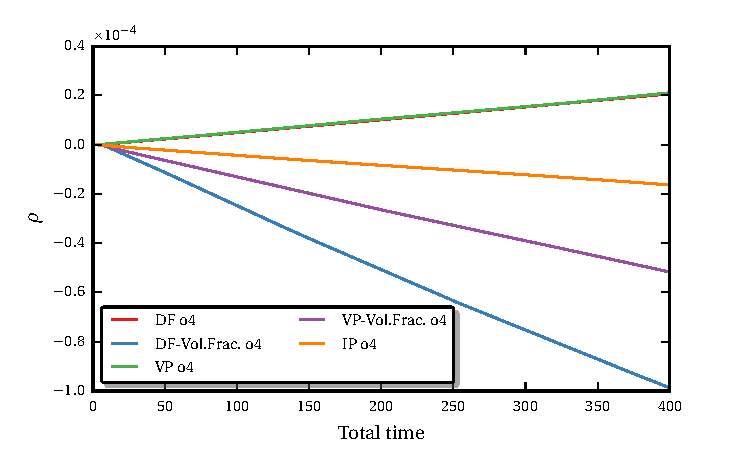
\includegraphics{gfx/immersed_boundary/hpflow/long/ts.pdf}
      \caption{\label{hpflow:results_long_ts}
            Averaged density for FD4 methods with respect to the simulation time.
          }
  \end{minipage}
  \hfill
  \begin{minipage}[c]{0.45\textwidth}
      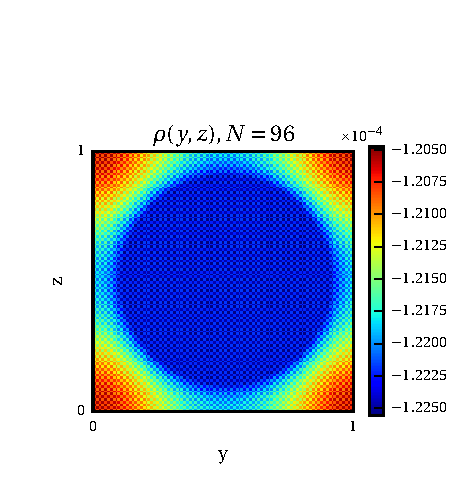
\includegraphics{gfx/immersed_boundary/hpflow/long/example.pdf}
      \caption{\label{hpflow:results_long_example}
        Density in the (y, z) plane, at $T_{\text{end}}=1600$, for the VP-VF-FD4 method.
      }
  \end{minipage}
\end{figure}

\clearpage
\subsection{Taylor-Couette Flow}

\subsubsection{Grid Convergence Study}


The results of the grid convergence study are shown from Fig. \ref{vali:tc_flow_gc_vp} to Fig. \ref{vali:tc_flow_gc_all}.
For a better overview the results are distributed into four plots.

In Fig. \ref{vali:tc_flow_gc_vp} the relative $l_2$-error is shown for different VP methods.
For the VP FD2 method the error convergence rate is about $\lambda=1.07$,
for the VP FD4 method it is about $\lambda=1.16$. However, it can be seen that the convergence rates decrease above $N\approx100$.
In this interval the error of the VP FD4 method remains approximately constant.
The VP-VF methods have a larger error (about $5\cdot 10^{-2}$ at $N=100$) in comparison the VP methods (about $0.9 \cdot 10^{-3}$ and  $2\cdot10^{-2}$ at $N=100$).
In contrast a higher convergence can be observed (about $\lambda=1.3$) for the VP-VF methods.

In Fig. \ref{vali:tc_flow_gc_df} the relative $l_2$-error is shown for different DF methods.
For all methods the error convergence rate is about first order, except the DF FD4 method which is about $\lambda=0.9$ .
The smallest error is given by the DF FD2 method which is about $2 \cdot 10^{-2}$ for $N=100$.
In comparison the error of the remaining methods is about $5\cdot10^{-2}$.

In Fig. \ref{vali:tc_flow_gc_ip} the relative $l_2$-error is shown for different IP methods.
For the IP FD4 method the convergence rate is about $\lambda=1.47$.
For the IP FD2 and IP+DF FD2 method the errors are nearly  identical, the convergence above first order.
The IP+DF FD4 method is numerically not stable and  not shown.
From the interpolation methods the IP-FD4 method gives the smallest error for $N>100$ which is of order $10 \cdot 10^{-3}$.
Again it can be seen that the convergence rate decreases above $N\approx100$ for all methods.

%For all methods, except IP+DF-FD4) an approximately linear decrease in the double logarithmic space can be observed.
%In summary it can be said that the overall convergence rate of the IP-FD2-method is of one order better
%than the VP-VF and DF-VF methods. The relative error of the interpolation method ranges
%between one and two order of magnitudes below all other methods, depending on the resolution.

Finally Fig. \ref{vali:tc_flow_gc_all} shows the methods with the best convergence
rates from the different DF, VP and IP methods in one plot.
It can be noted that in this validation the errors are not decreasing linearly in the log-log space.
The best results are given by the interpolation methods with small differences in the overall error
and convergence rates.

\subsubsection{Differences in the Velocity Profiles}

Beside the computation of the relative $l_2$-error, the local difference between the theoretical and numerical velocity
profile was computed by subtracting the vector fields from each other in the $(x, y)$ plane for a constant $z$
\footnote{Since $\partial_z \vec{v} = 0$ an arbitrary $z$ value can be used, i.e. $z=0$}.
The results for the FD2 schemes are presented in Fig. \ref{tcflow:results_vprofiles_o2}. The profiles
for the FD4 schemes are shown in the Appendix in Fig. \ref{tcflow:results_vprofiles_o4}.
From the profiles it can be noted that for all methods the difference between the numerical and
theoretical solution are the largest at the boundary $r_i$ of the  inner cylinder.
In this region the error is of order $10^{-2}$ for all methods.

\clearpage
\begin{figure}[!bp]
  \begin{minipage}[c]{0.45\textwidth}
      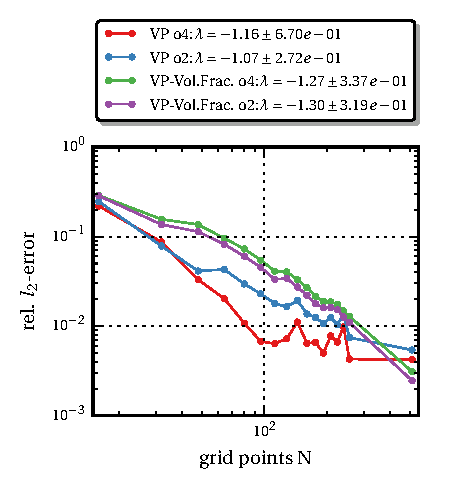
\includegraphics{gfx/immersed_boundary/tcflow/theo/vp.pdf}
      \caption{Relative $l_2$-error for different Volume-Penalization methods.}
      \label{vali:tc_flow_gc_vp}
  \end{minipage}
  \hfill
  \begin{minipage}[c]{0.45\textwidth}
      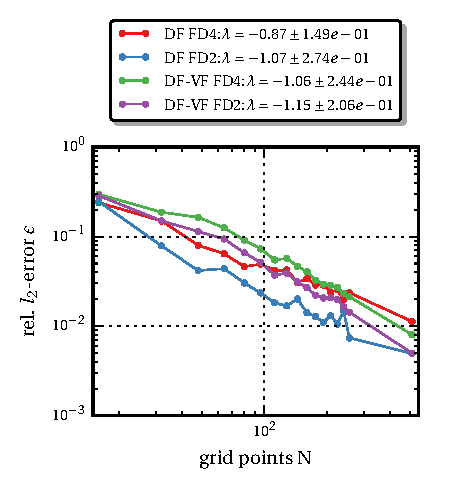
\includegraphics{gfx/immersed_boundary/tcflow/theo/df.pdf}
      \caption{Relative $l_2$-error for different Direct-Forcing methods.}
      \label{vali:tc_flow_gc_df}
  \end{minipage}

  \begin{minipage}[c]{0.45\textwidth}
      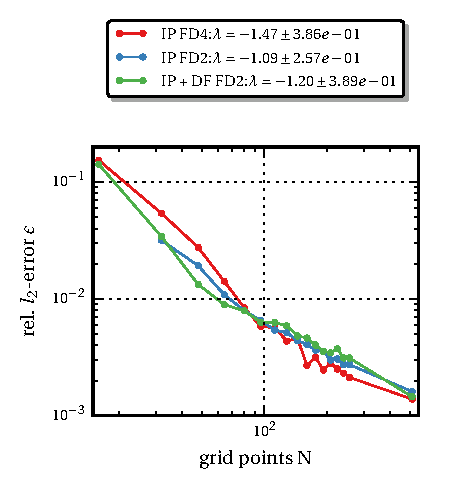
\includegraphics{gfx/immersed_boundary/tcflow/theo/ip.pdf}
      \caption{Relative $l_2$-error for different Interpolation methods.}
      \label{vali:tc_flow_gc_ip}
  \end{minipage}
  \hfill
  \begin{minipage}[c]{0.45\textwidth}
      \includegraphics{gfx/immersed_boundary/tcflow/theo/all.pdf}
      \caption{Relative $l_2$-error for the methods with the smallest error in comparison.}
      \label{vali:tc_flow_gc_all}
  \end{minipage}
\end{figure}
\clearpage

\begin{figure}[!bp]
  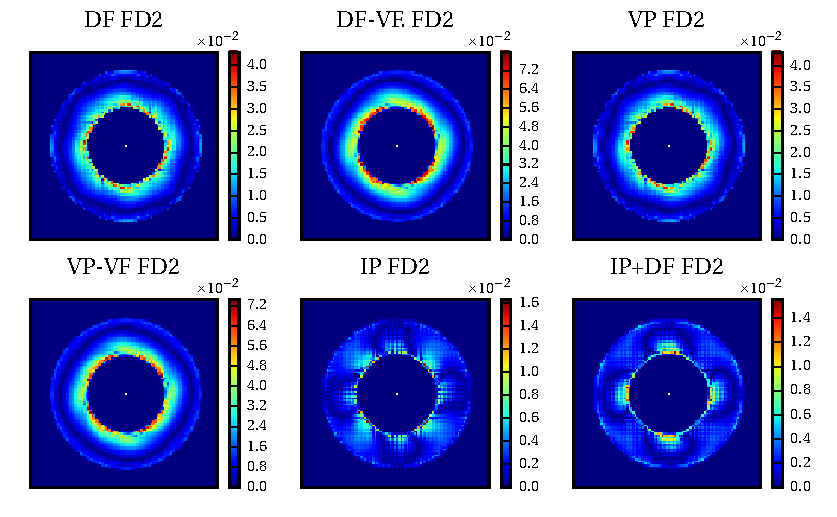
\includegraphics{gfx/immersed_boundary/tcflow/long/vz_profiles_o2.pdf}
  \caption{\label{tcflow:results_vprofiles_o2}
    Subtraction of the numerical velocity profile from the theoretical
        for all FD2 methods.}
\end{figure}

\begin{figure}[!bp]
  \begin{minipage}[c]{0.45\textwidth}
      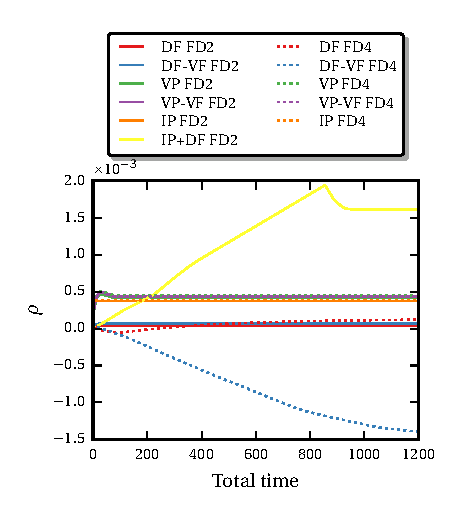
\includegraphics{gfx/immersed_boundary/tcflow/long/ts_all.pdf}
      \caption{\label{tcflow:results_long_ts_o2}
            Averaged density for all methods with respect to the simulation time.
          }
  \end{minipage}
  \hfill
  \begin{minipage}[c]{0.45\textwidth}
      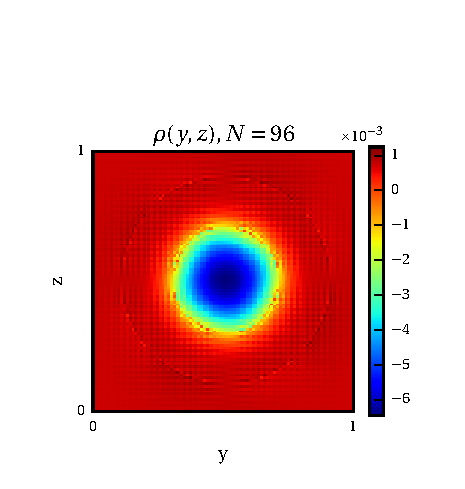
\includegraphics{gfx/immersed_boundary/tcflow/long/example.pdf}
      \caption{\label{tcflow:rho_example}
        Density oscillations for the VP-VF FD2 method with a decreased density in the inner cylinder.
      }
  \end{minipage}
\end{figure}

\clearpage

\subsubsection{Long-Term Simulations}

For all methods the simulations were numerically stable, except the IP FD4 method.
The density was averaged over the fluid domain by Eq. \ref{vali:density_calc},
the results of the computation are shown in Fig. \ref{tcflow:results_long_ts_o2}.
For the IP+DF FD2 method the density increases from zero until a convergence is reached at $T\approx 1000$ of about $1.6\cdot10^{-3}$.
The density of the  DF-VF FD4 decreases to $-1.4\cdot10^{-3}$ with a convergence at $T\approx1400$.
For all other methods a faster convergence is reached at $T\approx200$ with an  averaged density in the order $10^{-4}$.

For all methods numerical oscillations in the density can be
observed, which  are similar to the Hagen-Poiseuille flow test case.
In Fig. \ref{tcflow:rho_example} these oscillations are exemplarily shown for the VP-VF FD2 method.
In Appendix \ref{tcflow:results_rho_profiles_o2} the remaining FD2 methods are presented.
Besides these oscillations of order $10^{-4}$ it can be noted that the density in the inner cylinder
where the VP method is applied decreases to about $-6\cdot10^{-3}$, in contrast to $\approx10^{-3}$ in the fluid domain.

